\documentclass[tikz,border=10pt]{standalone}
\usepackage{tikz}
\usetikzlibrary{shapes,arrows,positioning}

\begin{document}
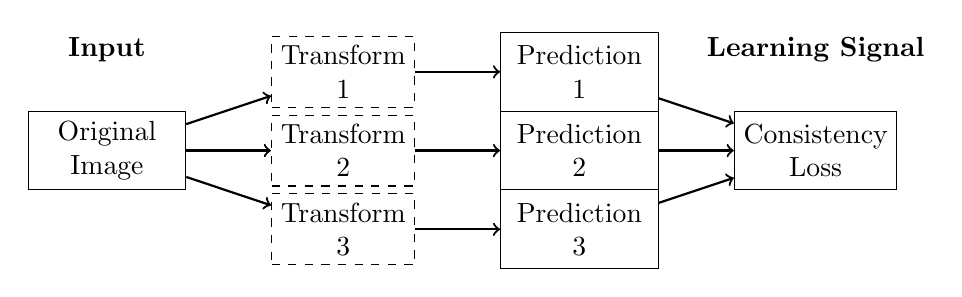
\begin{tikzpicture}[
    node distance=2cm,
    box/.style={rectangle, draw, minimum width=2cm, minimum height=1cm, align=center},
    arrow/.style={->, thick},
    transform/.style={rectangle, draw, dashed, minimum width=1.5cm, minimum height=0.8cm, align=center}
]

% Original image
\node[box] (original) at (0,0) {Original\\Image};

% Transformations
\node[transform] (transform1) at (3,1) {Transform\\1};
\node[transform] (transform2) at (3,0) {Transform\\2};
\node[transform] (transform3) at (3,-1) {Transform\\3};

% Model predictions
\node[box] (pred1) at (6,1) {Prediction\\1};
\node[box] (pred2) at (6,0) {Prediction\\2};
\node[box] (pred3) at (6,-1) {Prediction\\3};

% Consistency check
\node[box] (consistency) at (9,0) {Consistency\\Loss};

% Arrows
\draw[arrow] (original) -- (transform1);
\draw[arrow] (original) -- (transform2);
\draw[arrow] (original) -- (transform3);
\draw[arrow] (transform1) -- (pred1);
\draw[arrow] (transform2) -- (pred2);
\draw[arrow] (transform3) -- (pred3);
\draw[arrow] (pred1) -- (consistency);
\draw[arrow] (pred2) -- (consistency);
\draw[arrow] (pred3) -- (consistency);

% Labels
\node[above=0.5cm of original] {\textbf{Input}};
\node[above=0.5cm of consistency] {\textbf{Learning Signal}};

\end{tikzpicture}
\end{document}
